%%%%%%%%%%%%%%%%%%%%%%%%%%%%%%%%%%%%%%%%%%%%%%%%%%%%%%%%%%%%%%%%%%%%%%
% This document uses the LaTeX class file "article.cls"              %
%%%%%%%%%%%%%%%%%%%%%%%%%%%%%%%%%%%%%%%%%%%%%%%%%%%%%%%%%%%%%%%%%%%%%%
\documentclass[8pt,a4paper,twocolumn]{article}

%%%%%%%%%%%%%%%%%%%%%%%%%%%%%%%%%%%%%%%%%%%%%%%%%%%%%%%%%%%%%%%%%%%%%%
% Document preamble
%%%%%%%%%%%%%%%%%%%%%%%%%%%%%%%%%%%%%%%%%%%%%%%%%%%%%%%%%%%%%%%%%%%%%%

%% Builds upon the graphics  package, providing a key-value interface
%% for optional arguments to the \includegraphics command that go far
%% beyone what the graphics package offers.
%% http://www.ctan.org/tex-archive/help/Catalogue/entries/graphicx.html
%% if you use PostScript figures in your article
%% use the graphics package for simple commands
%% \usepackage{graphics}
%% or use the graphicx package for more complicated commands
%% \usepackage{graphicx}
%% or use the epsfig package if you prefer to use the old commands
%% \usepackage{epsfig}
\usepackage{graphicx} % Enhanced LaTeX Graphics
\usepackage{siunitx}

\graphicspath{{images/}}

%Tipo de letra Arial
\usepackage{helvet}
\renewcommand{\familydefault}{\sfdefault}

% acentos e cedilhas
\usepackage[utf8]{inputenc}
%\usepackage[T1]{fontenc}

% Multiple figures
%\usepackage{subfigure} % subcaptions for subfigures
%\usepackage{subfigmat} % matrices of similar subfigures

\usepackage[font=footnotesize, skip = 1pt, labelfont=bf]{caption}
\usepackage[font=footnotesize]{subcaption}

% Declaring new column types
% 'dcolumn' package defines D to be a column specifier with
% three arguments: D{<sep.tex>}{<sep.dvi>}{<decimal places>}
%                  D{<sep.tex>}{<sep.dvi>}{<left digit places>.<right digit places>}
\usepackage{dcolumn}           % decimal-aligned tabular math columns
% d takes a single argument specifying the number of decimal places, e.g., d{2}
% or the number of digits to the left and right of the seperator, e.g., d{3.2}
\newcolumntype{.}   {D{.}{.}{-1}} % column alignedd on the point separator '.'
\newcolumntype{d}[1]{D{.}{.}{#1}} % column centered on the point separator '.'
\newcolumntype{e}   {D{E}{E}{-1}} % column centered on the exponent 'E'
\newcolumntype{E}[1]{D{E}{E}{#1}} % column centered on the exponent 'E'

%% American Mathematical Society (AMS) plain Tex macros
%%
%% The amsmath package is the principal package in the AMS-LaTeX distribution
%% http://www.ctan.org/tex-archive/help/Catalogue/entries/amsmath.html
\usepackage{amsmath}
\DeclareMathSizes{7}{7}{3}{3} 
\usepackage{pifont}
%%
%% The amsfonts package provides extended TeX fonts
%% http://www.ctan.org/tex-archive/help/Catalogue/entries/amsfonts.html
\usepackage{amsfonts}
%% The amssymb package provides various useful mathematical symbols
\usepackage{amssymb}
%%
%% The amsthm package provides extended theorem environments
%% http://www.ctan.org/tex-archive/help/Catalogue/entries/amsthm.html
\usepackage{amsthm}
\usepackage{multirow}
%% Improves the interface for defining floating objects such as figures and tables.
%% The package also provides the H float modifier option of the obsolete here package.
%% http://www.ctan.org/tex-archive/help/Catalogue/entries/float.html
\usepackage{float}

%% Control sectional headers. 
%% http://www.ctan.org/tex-archive/help/Catalogue/entries/sectsty.html
\usepackage{sectsty}
%%
%% Redefine the font size of the 'section' and 'subsection' headings
\newcommand{\myFontSize}{\fontsize{9}{0}\selectfont}
\sectionfont{\myFontSize}       % 10pt, Bold face (default)
\subsectionfont{\myFontSize} % 10pt, Plain face

%% Select alternative section titles.
%% http://www.ctan.org/tex-archive/help/Catalogue/entries/titlesec.html
\usepackage{titlesec}
\usepackage{booktabs}
%\usepackage{multirow}
%\usepackage{array}
\usepackage{csquotes}% Recommended
%\usepackage[style=authoryear, backend=bibtex, doi=false,isbn=false,url=false,eprint=false,dashed=false,maxcitenames=2, maxbibnames=100]{biblatex}
%\addbibresource{library.bib}

%%
%% Left indent, before and after spacing
%% (The starred version kills the indentation of the paragraph following the title)
\titlespacing*{\section}{0pt}{10pt}{0pt}
\titlespacing*{\subsection}{0pt}{10pt}{0pt}

%% Section numbers with trailing dots. 
%% http://www.ctan.org/tex-archive/help/Catalogue/entries/secdot.html
\usepackage{secdot}
\usepackage{epstopdf}
%%
%% Also put a dot after the subsection number
\sectiondot{subsection}
%% Set a space between dot and heading text
\sectionpunct{section}{. }    % By default, \sectiondot places a \quad
\sectionpunct{subsection}{. } % after the number

% These are exact settings for a A4 page with top margin of
% 25 mm, bottom margin of 30 mm, left and right margins of 25 mm,
% printable area 242 X 160 mm.

\setlength{\topmargin}{-10.4mm}
\setlength{\headheight}{0.0mm}
\setlength{\headsep}{10.0mm}
\setlength{\textwidth}{160mm}
\setlength{\textheight}{242mm}
\setlength{\oddsidemargin}{0mm}
\setlength{\evensidemargin}{0mm}
\setlength{\marginparwidth}{0mm}
\setlength{\marginparsep}{0mm}

% New command to refer to equations as Eq.(1),Eq.(2),...
\newcommand{\eqnref}[1]{Eq.(\ref{#1})}

%%%%%%%%%%%%%%%%%%%%%%%%%%%%%%%%%%%%%%%%%%%%%%%%%%%%%%%%%%%%%%%%%%%%%%%%%%%%%%%%%%%%%%%%
% Title, authors and addresses

\title{\bfseries Twitter Sentiment Analysis - Support Vector Machine}
\date{December 2019}
\author{Daniele Gerbaldo, Thieu Nguyen, Tim Röthig \\ daniele.gerbaldo.001@student.uni.lu,\\ thieu.nguyen.001@student.uni.lu,\\ tim.roethig.001@student.uni.lu \\ \\University of Luxembourg,\\ Faculty of Science, Technology and Communication
}

%%%%%%%%%%%%%%%%%%%%%%%%%%%%%%%%%%%%%%%%%%%%%%%%%%%%%%%%%%%%%%%%%%%%%%%%%%%%%%%%%%%%%%%%
\begin{document}

% Begin one column section for title and abstract
%
% http://www.faqs.org/faqs/de-tex-faq/part5/
\twocolumn[
\begin{@twocolumnfalse}
\maketitle

	%%%%%%%%%%%%%%%%%%%%%%%%%%%%%%%%%%%%%%%%%%%%%%%%%%%%%%%%%%%%%%%%%%%%%%
%     File: ExtendedAbstract_abstr.tex                               %
%     Tex Master: ExtendedAbstract.tex                               %
%%
%% Abstract
%%
\begin{abstract}
Sentiment analysis refers to the use of machine learning, natural language processing, and computational linguistics to determine the sentiment content from the written language, i.e. it analyzes people's opinions, attitudes, and emotions for products, services, organizations, individuals, events or topics. In this project, we try to build the automatic sentiment analyzer system based on SVM and other techniques. The frequency of occurrence of words used as features for SVM. To evaluate our system, the Twitter dataset which containing tweets that are manually annotated for the sentiment (positive, negative or neutral) will be used. Eventually, we use the system to classify the unseen message's sentiments. \\

%%
%% Keywords (max 5)
%%
\noindent{{\bf Keywords:}} Machine Learning, Sentiment Analysis, SVMs, Feature Selection, Twitter Dataset, Nature Language Processing \\

\end{abstract}



\end{@twocolumnfalse}
]
	\section{Introduction}
\label{sec:intro}

Nowadays, the age of the Internet has changed the way people express their opinions and views.  It is now mainly done through blog posts, online forums, product review websites, social media, etc. Millions of people are using social network sites like Facebook, Twitter, Google Plus, etc. to express their feelings, opinion and share views about their daily lives. Social media is generating a massive amount of sentiment data in the form of tweets, status updates, blog posts, comments, reviews, etc.  Therefore, It is provided an opportunity for businesses by giving a platform to connect with their customers for advertising. People mostly depend on user-generated content online to a large extent to make decisions. For example, if someone wants to buy a product or wants to use any service, they firstly search for its reviews online, discuss it on social media before making a decision. The amount of content generated by users is too large for the normal user to analyze. Therefore, it is necessary to automate this, various sentiment analysis techniques are widely used. Sentiment analysis influences users to classify whether the information about the product is satisfactory or not before they acquire it. Marketers and firms use this analysis to understand their products or services in such a way that it can be offered as per the user’s needs.

There are two types of machine learning techniques that are generally used for sentiment analysis, one is unsupervised and the other is supervised. Unsupervised learning does not consist of a category and they do not provide with the correct targets at all and therefore conduct clustering. Supervised learning is based on the labeled dataset and thus the labels are provided to the model during the process. These labeled datasets are trained to produce reasonable outputs when encountered during decision- making. 

To help us to understand the sentiment analysis in a better way, this project is based on supervised machine learning. The rest of the paper is organized as follows. The second section discusses in brief about the work carried out for sentiment analysis in the different domain by various researchers. The third section is about the approach we followed for sentiment analysis. Section four is about implementation details and results followed by a conclusion and future work discussion in the last section. 

	% A Theory section should extend, not repeat, the background to the
% article already dealt with in the Introduction and lay the
% foundation for further work.

\section{Related Work}
\label{sec: backg}

Work in the field "Sentiment analysis" has started since the beginning of the century. In its early stage, it was intended for binary classification, which assigns opinions or reviews to bipolar classes such as positive or negative. Paper \cite{turney2002thumbs} predicts review by the average semantic orientation of a phrase that contains adjectives and adverbs thus calculating whether the phrase is positive or negative with the use of unsupervised learning algorithm which classifies it as thumbs up or thumbs down the review. 
 
 In \cite{liu2011movie} the product feature uses a latent semantic analysis (LSA) based filtering mechanism to identify opinion words that are used to select some sentences to become a rich review summarization.  In another work \cite{khan2011sentiment}, the polarity of the word is being calculated by all the words in the sentence, which can either be positive or negative depending on the related sentence structure. In \cite{ramachandran2011automated} has proposed to pre-process the data to improve the quality structure of the raw sentence. They have applied the LSA technique and cosine similarity for sentiment analysis. \cite{karamibekr2012verb} proposed a method based on verbs as an important opinion term for sentiment classification of a document belonging to the social domain. In \cite{agarwal2013sentiment} applied phrase pattern method for sentiment classification. It uses part of speech based rules and dependency relation for extracting contextual and syntactic information from the document. 

Overall, a lot of work has also been done where researchers have explored and applied soft-computing approaches, mainly machine learning and neural works for sentiment analysis. In \cite{go2009twitter}, the authors introduce a novel approach for automatically classifying the sentiment of Twitter messages. Their main idea is using tweets with emoticons for distant supervised learning. They apply several machine learning algorithms like Naive Bayes, Maximum Entropy, and SVM. In \cite{gautam2014sentiment}, the authors applied several ML techniques like Naive Bayes, Maximum entropy and SVM along with the Semantic Orientation based WordNet which extracts synonyms and similarity for the content feature to analyze customer's review sentiment. 











	\section{Methodology}
\label{sec: Methodology}
% In this section. First, we describe the dataset. Second we show how we collecting data, preprocessing data for the model and the last we describe our algorithm.


A dataset is created using twitter (a popular micro-blogging service where users create status messages called tweets) posts of electronic products. These tweets sometimes express opinions about different topics. Therefore, they are short messages full of slang words and misspellings (Fig.\ref{fig1}).  So we propose a method to automatically classifying sentiment (positive or negative) from a tweet. This is done in three phases. In the first phase preprocessing is done. Then a feature vector is created using relevant features. Finally using SVM classifiers, tweets are classified into positive and negative classes. 

\begin{figure*}[!htb]
    \center{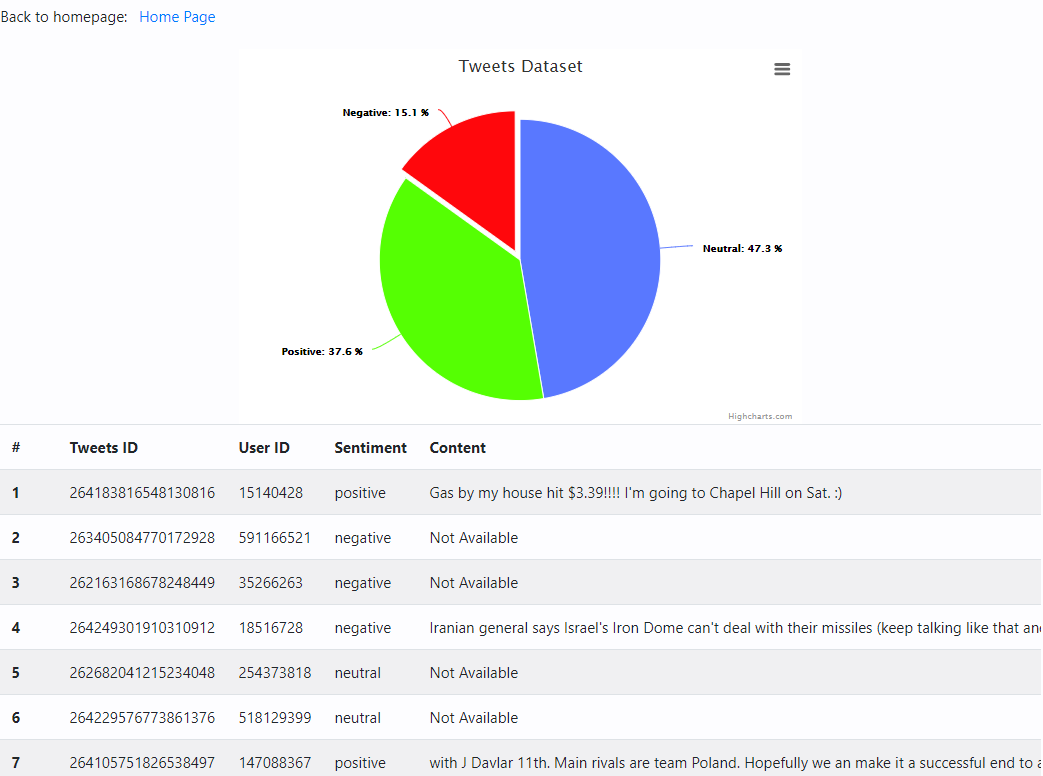
\includegraphics[width=1.4\columnwidth]{original_dataset.png}}
    \caption{\label{fig1} Original dataset}
\end{figure*}

\begin{figure*}[!htb]
    \center{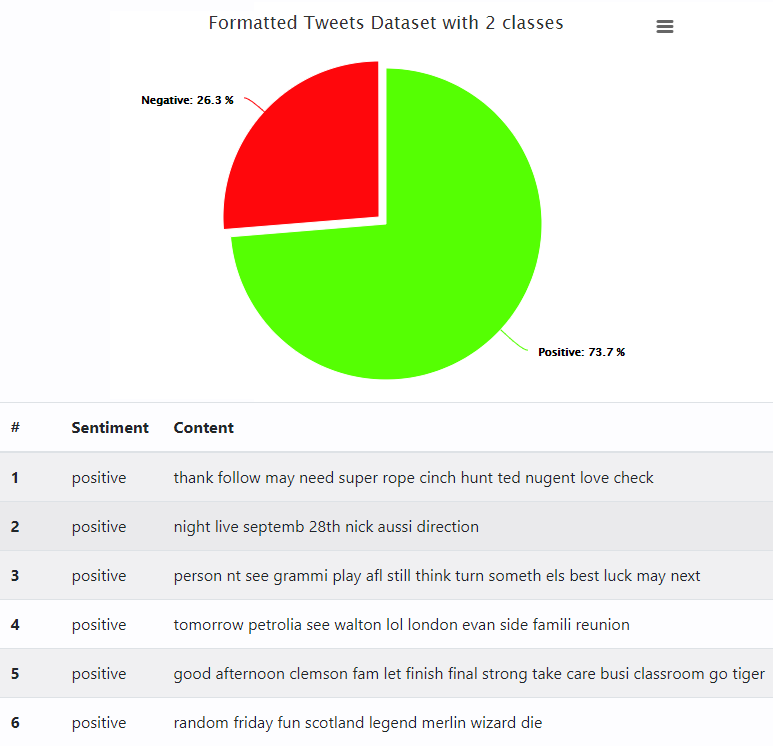
\includegraphics[width=1.4\columnwidth]{formatted_2classes.png}}
    \caption{\label{fig3} Our dataset after preprocessing}
\end{figure*}


\subsection{Dataset}
\label{sec: Dataset}

The data used in this project for training and testing is SemEval-2014 Twitter dataset Task 9 Corpus \cite{nakov2016evaluation} which was collected within the SemEval-2014 Task 9 competition that was a part of the International Workshop on Semantic Evaluation. We used 80$\%$ of the dataset for training and the remaining 20$\%$ for testing.


\subsection{Preprocessing Data}
\label{sec: Preprocessing Data}

A tweet contains a lot of opinions about the data which are expressed in different ways by different users. So keyword extraction is difficult on twitter due to misspellings and slang words. To avoid this, a preprocessing step is performed before feature extraction. Preprocessing steps include several techniques following to select features from the raw data: 

\begin{itemize}
    \item Remove all URLs (e.g. $www.xyz.com$), hash tags (e.g. $\#topic$), targets ($@$username), hyperlinks, numbers, repeated letters (more than 2 repeated letters) and punctuation marks.
    \item Removing stop words that add no sentiment value (articles, some prepositions, etc.).
    \item Stemming: reducing distinct words to their root form (stem).
    \item Removing infrequent words (words that appear less than $n_{min}$ number of times).
\end{itemize}

\subsection{Creation of Feature Vector}
\label{sec: Creation of Feature Vector}
 

\begin{figure}[!ht]
    \center{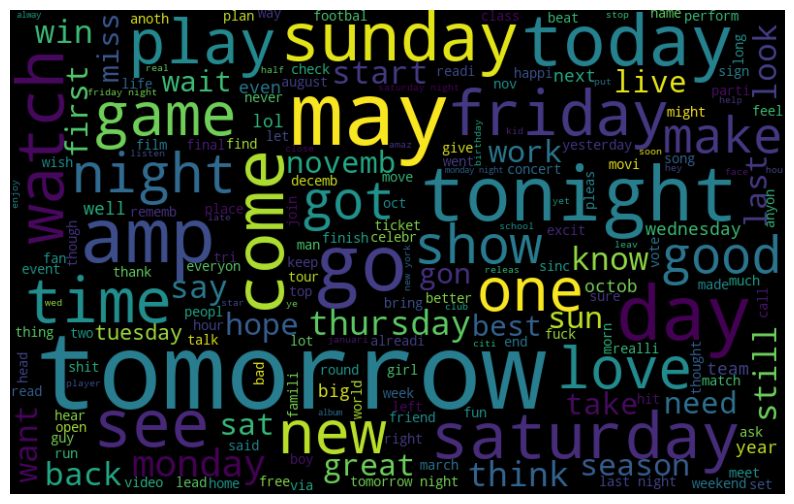
\includegraphics[width=1.0\columnwidth]{features.png}}
    \caption{\label{fig_feature_vector} Our features}
\end{figure}


For the unigram feature, there are usually a larger 500,000 different features. This is a very large number. It makes a model a higher variance. (Since the more complicated model has higher variance). It will need much more training data to avoid overfitting. Our dataset set contains almost 10 hundreds of sentences. This is a small number of examples. So we need to discard some useless features.

In this project, we use frequency-based feature selection which is the simplest way to do the feature selection. We just pick features (unigram words in our case) for each class with high-frequency occurrence in this class. In practice, if the number of occurrences of a feature is larger than some threshold (100 or 1000 in our experiments), this feature is a good one for that class (Fig.\ref{fig_feature_vector}). As we have seen in the result table, this simple algorithm increases about 0.03 of accuracy.



\subsection{Classification Technique}
\label{sec: Classification Technique}

There are different types of classifiers that are generally used for text classification which can be also used for twitter sentiment classification. But in this project, we focus on using  Support Vector Machine to do classify twitter sentiment.

SVM Classifier uses a large margin for classification. It separates the tweets using a hyperplane. SVM uses the discriminative function defined as

\begin{equation} \label{eq: svm}
g(X) = w^T \phi(X) + b
\end{equation}

$X$ is the feature vector, $w$ is the weights vector and $b$ is
the bias vector. $\phi()$ is the non-linear mapping from input space to high dimensional feature space. $w$ and $b$ are learned
automatically on the training set. Here we used different kernels for classification such as linear and radial basis functions. It maintains a wide gap between two classes.


\subsection{Automated Sentiment Classification System}
\label{sec: system}

After the training and testing process, we selected and saved the best model for later usage. After that, we built a web interface tool to aid in the manual user-defined query and then automated sentiment classification. 
 
After typing the user-query (query will be directly done by Twitter API).  The saved model is loaded and used to classify the tweets (return from twitter api). The statistics of the number of positive and negative tweets also are also calculated. The classification labels is compared between our model and TextBlob (\cite{loria2014textblob}) model (Fig.\ref{automated_system}).

\begin{figure*}[!t]
    \center{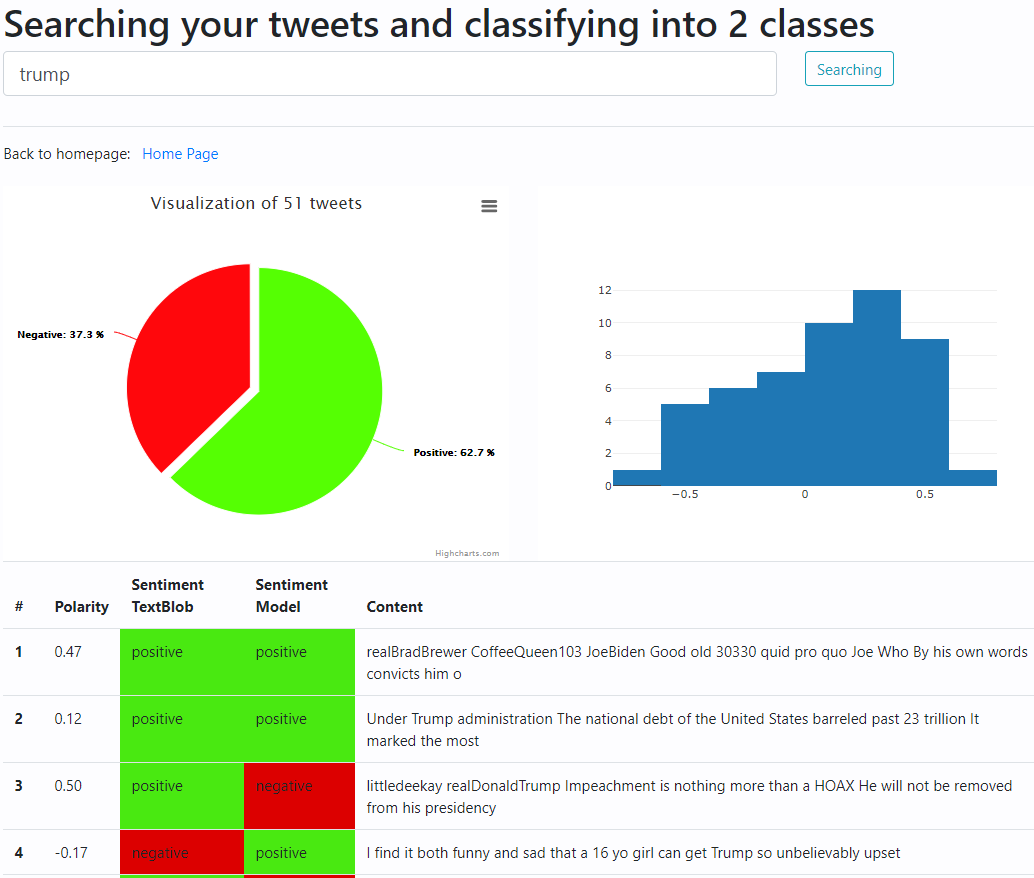
\includegraphics[width=1.8\columnwidth]{searching_and_comparing.png}}
    \caption{\label{automated_system} Automated sentiment classification system}
\end{figure*}



	\section{Results \& discussion}
\label{sec:resul}

We have not mentioned the polynomial function due to the factor that is always performing worst in our tests.
In the following table you can see the result for linear and Radial Basis function kernel type and different values of C.

\begin{table}[!ht]
	\begin{center}
	\begin{tabular}{ccc}
		\hline
		Kernel Type  & C & Accuracy  \\ 
		\hline
		\multirow{4}{*}{Radial Basis function}       & 0.5     & 75$\%$ \\
				 & 1        & 78 $\%$         \\
				 & 3        & 84  $\%$       \\
				 & 5        & 83 $\%$    	    \\
		\hline
		\multirow{4}{*}{Linear}       & 0.5     & 78$\%$ \\
				 & 1        & 80 $\%$         \\
				 & 3        & 82  $\%$       \\
				 & 5        & 77 $\%$    	    \\ \hline
	\end{tabular}
	\end{center}
	\caption{Summary of accuracy with different kernel and different C.}
	\label{tb:table2}
\end{table}	

Another important parameter to tune was the minimum word frequency. The following table contains evaluation of different word frequencies.


\begin{table}[!ht]
	\begin{center}
	\begin{tabular}{cc}
		\hline
		Word Freequency & Accuracy  \\ 
		\hline
		3      & 75$\%$ \\
				5  & 79 $\%$         \\
				   7 & 77  $\%$       \\
				 10    & 76 $\%$    	    \\
		\hline
	\end{tabular}
	\end{center}
	\caption{Summary of accuracy with different kernel and different C.}
	\label{tb:table3}
\end{table}	



Based on this knowledge we chose the following hyper-parameters:


\begin{table}[!h]
	\begin{center}
	\begin{tabular}{c | c}
		\hline
		Word Freequency & 5 \\ \hline 
		
		
		Kernel Type & Radial Basis \\  \hline 
		
		C & 3 \\  \hline 
		
		Training Accuracy & 95$\%$ \\  \hline 
		
		Test Accuracy & 85$\%$ \\ 
		\hline
	\end{tabular}
	\end{center}
	\caption{Summary of accuracy with different kernel and different C.}
	\label{tb:table4}
\end{table}	
	\section{Conclusions}
\label{sec:concl}

The SVM has been widely used and promoted for land cover classification studies. So in this project, we proposed the used of SVM with sentiment analysis for classifying the sentence based on twitter data. There are certain issues while dealing with misspellings and slang words from tweets. To deal with these issues, the efficient feature vector is created by doing preprocessing. After preprocessing the raw data, we aim to build an automatic sentiment system by using the twitter dataset which is already labeled. The classification accuracy of the model is tested using the SVM classifier but with a different configuration of parameters. Unigram model is deployed with SVM to classify the sentiment of Twitter data. The training data set can be increased to improve the feature vector related sentence identification process. It may give a better visualization of the content in a better manner that will be helpful for the users. A major conclusion of this study is that the accuracy of SVM classification is influenced by the number of features used.




% REFERENCES

% Produces the bibliography section when processed by BibTeX
%
% Bibliography style
% > entries ordered alphabetically
%\bibliographystyle{plain}
% > unsorted with entries appearing in the order in which the citations appear.
%\bibliographystyle{unsrt}
% > entries ordered alphabetically, with first names and names of journals and months abbreviated
\bibliographystyle{abbrv}
% > entries ordered alphabetically, with reference markers based on authors' initials and publication year
%\bibliographystyle{alpha}

% External bibliography database file in the BibTeX format (ExtendedAbstract_ref_db.bib)
\bibliography{references}

\end{document}


